\begin{flushright} {\tiny {\color{gray} python\_codes/fieldstone\_01/text.tex}} \end{flushright}

\lstinputlisting[language=bash,basicstyle=\small]{python_codes/fieldstone_01/keywords}

\begin{center}
Code at \url{https://github.com/cedrict/fieldstone/tree/master/python_codes/fieldstone_01}
\end{center}

\par\noindent\rule{\textwidth}{0.4pt}

{\sl This fieldstone was developed in collaboration with Job Mos}. \index{contributors}{J. Mos}

\par\noindent\rule{\textwidth}{0.4pt}
%%%%%%%%%%%%%%%%%%%%%%%%%%%%%%%%%%%%%%%%%%%%%%%%%%%%%%%%%%%%%%%%%%%%%%%%%%%%%%%%%%%%%%%%%%%%%%

This benchmark is taken from Donea \& Huerta (2003) \cite{dohu03} and is described fully in section \ref{mms1}. 
In order to illustrate the behavior of selected mixed finite elements in the solution 
of stationary Stokes flow,  we consider a two-dimensional problem 
in the square domain $\Omega=[0,1]\times[0,1]$, which possesses a closed-form analytical 
solution. 

\begin{center}
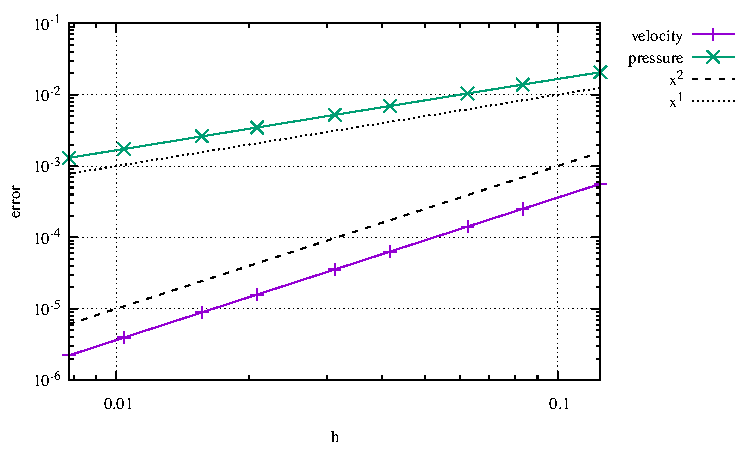
\includegraphics[width=10cm]{python_codes/fieldstone_01/results/errors.pdf}\\
{\captionfont Quadratic convergence for velocity error, 
linear convergence for pressure error, as expected.}
\end{center}

\begin{center}
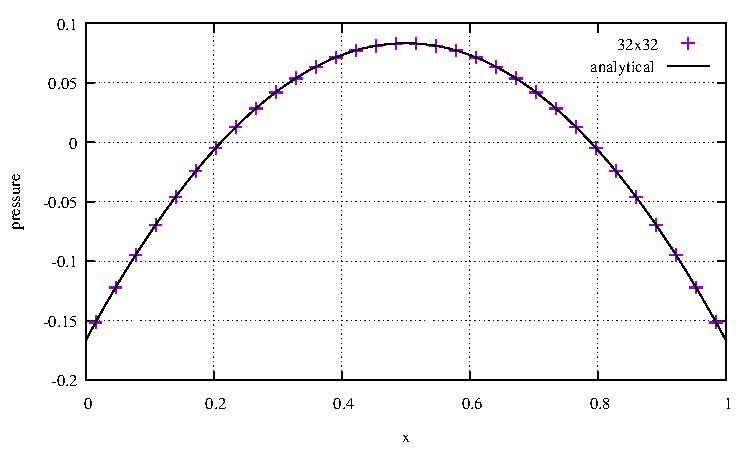
\includegraphics[width=10cm]{python_codes/fieldstone_01/results/pressure.pdf}\\
{\captionfont Pressure field}
\end{center}

\begin{center}
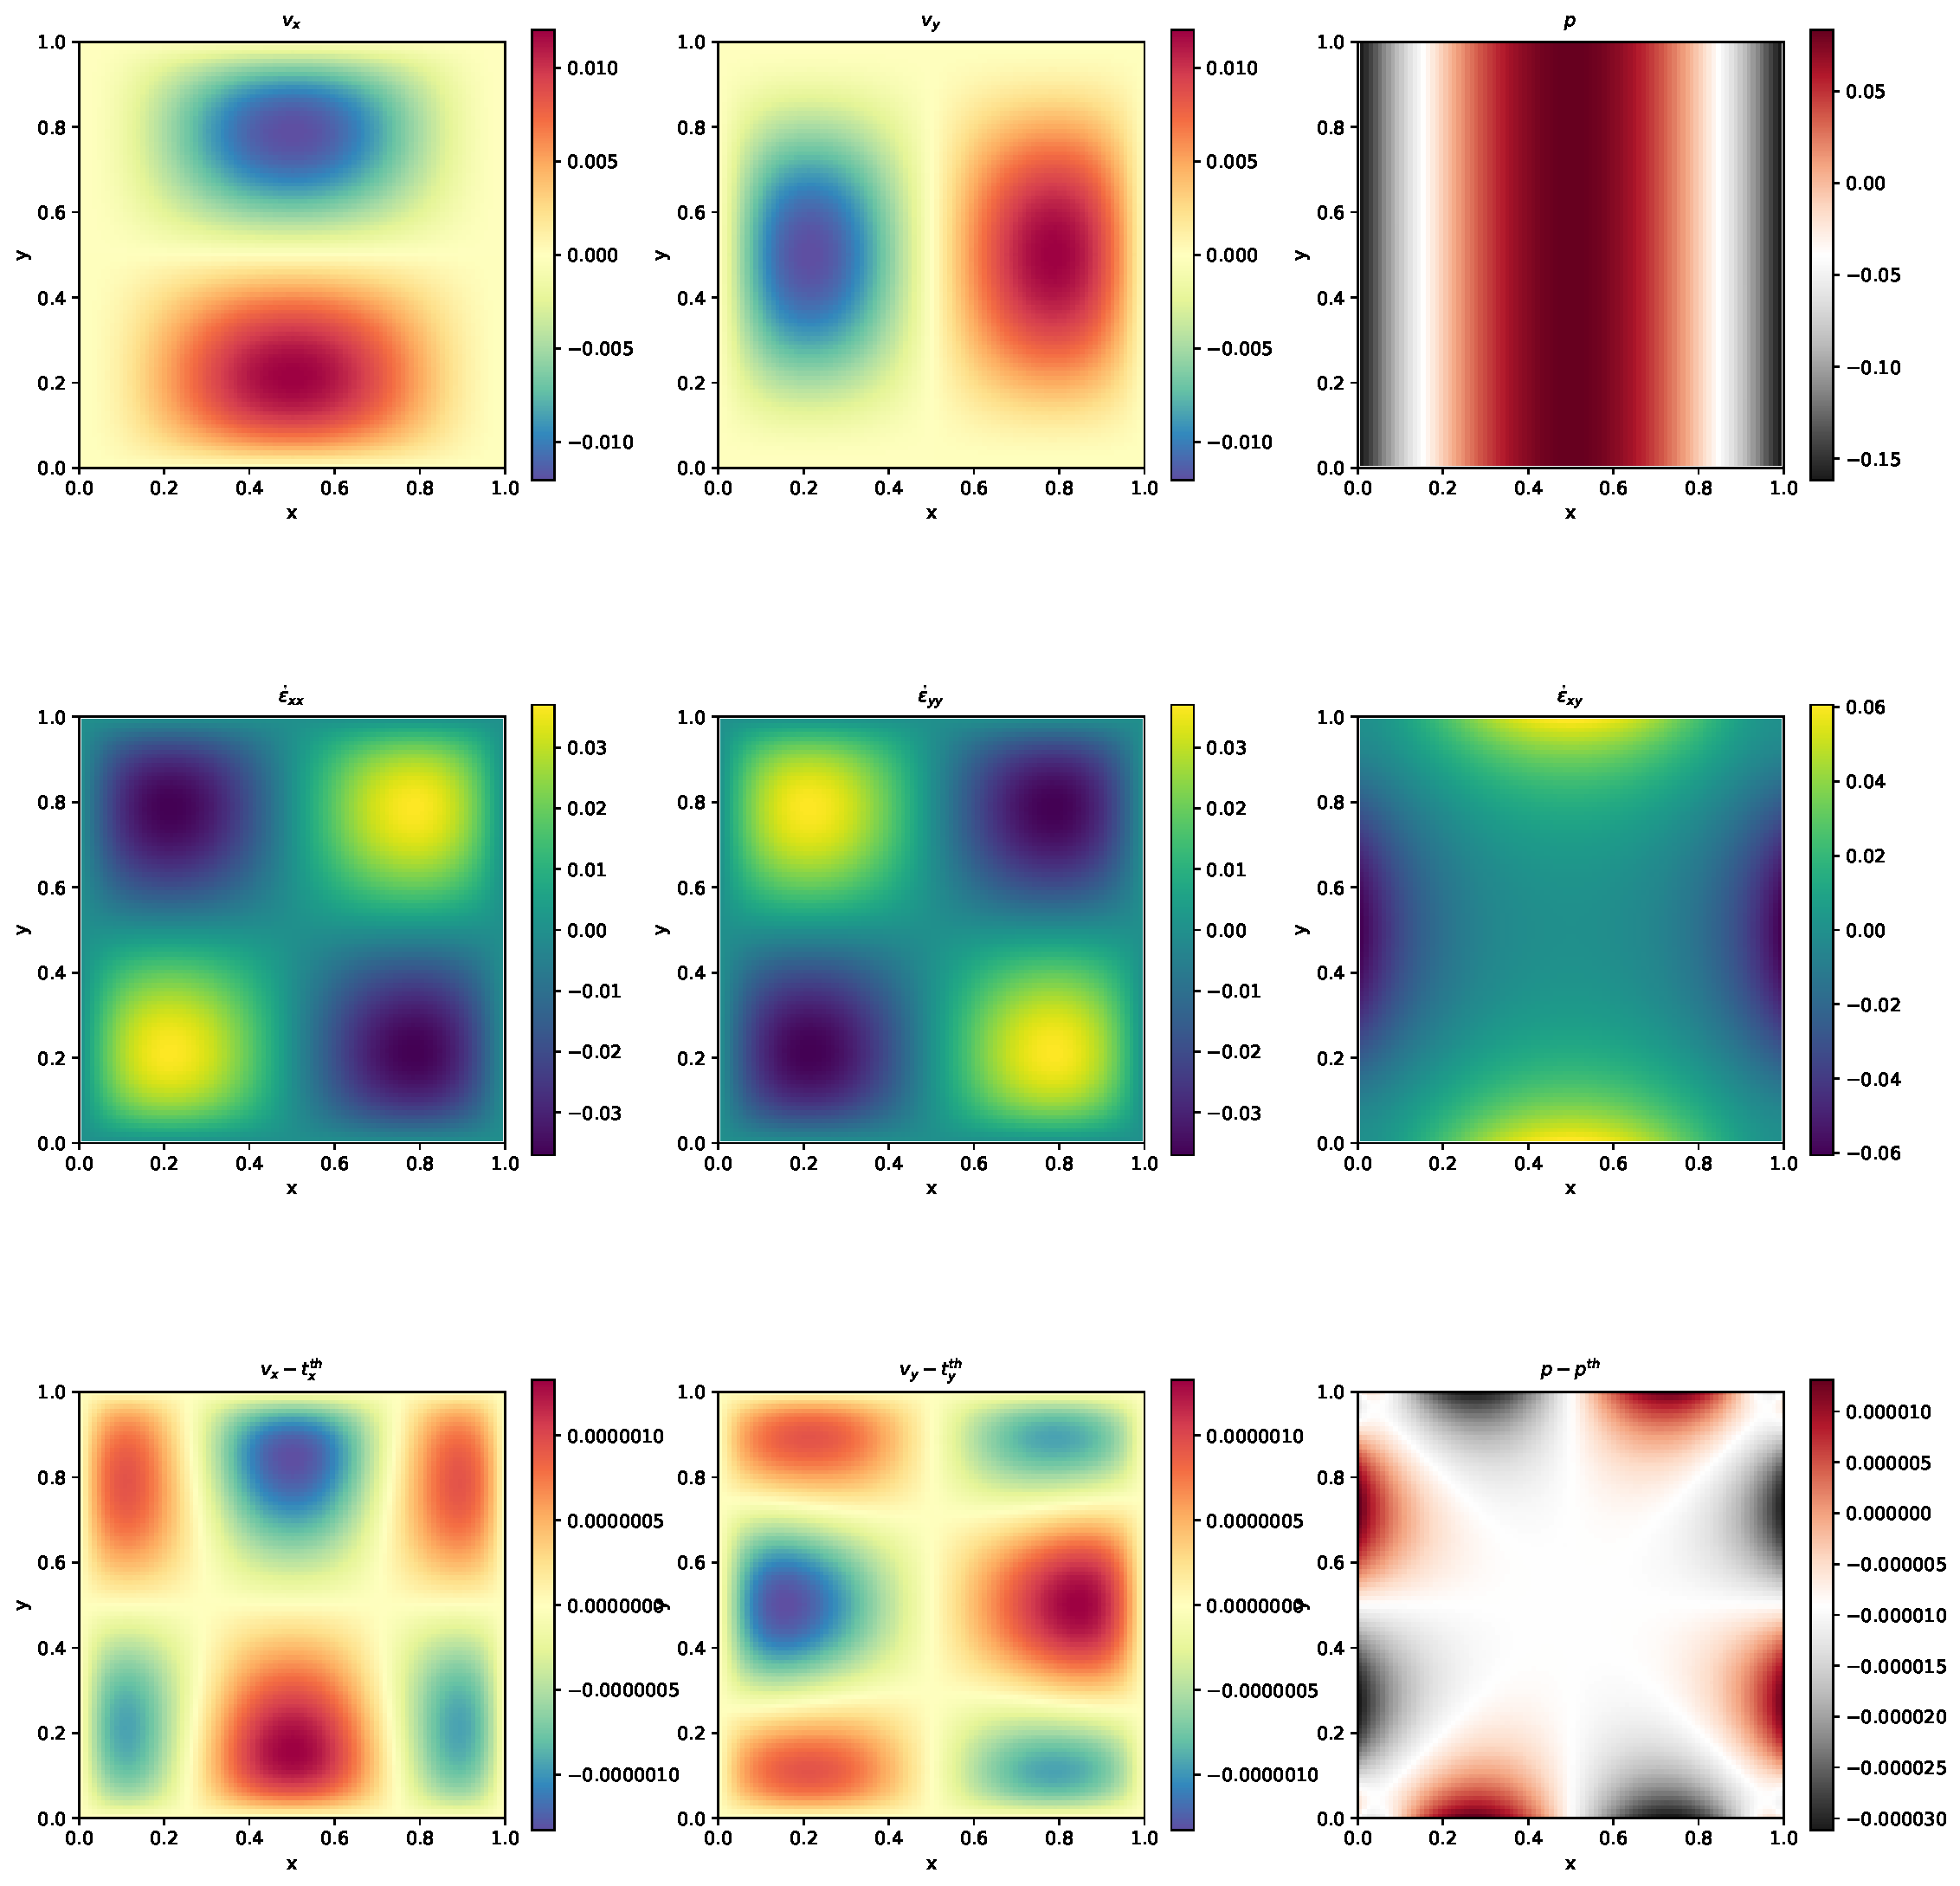
\includegraphics[width=15cm]{python_codes/fieldstone_01/solution.pdf}
\end{center}



\includegraphics[width=1cm]{images/fortran/fortran} I wrote the first ever version of this stone in
Fortran90 around 2011. It is available in the {\foldernamefont simplefem} folder in this stone.
\index{general}{fortran90}
